\documentclass[a4paper,twoside]{article}

\usepackage{epsfig}
\usepackage{subfigure}
\usepackage{calc}
\usepackage{amssymb}
\usepackage{amstext}
\usepackage{amsmath}
\usepackage{amsthm}
\usepackage{multicol}
\usepackage{pslatex}
\usepackage{apalike}
\usepackage{SCITEPRESS}     % Please add other packages that you may need BEFORE the SCITEPRESS.sty package.

\subfigtopskip=0pt
\subfigcapskip=0pt
\subfigbottomskip=0pt

\begin{document}

\title{Ontology Based Description of Analytic Methods for Electrophysiology}

\author{\authorname{Jan Stebetak\sup{1}, Roman Moucek\sup{2}}
\affiliation{\sup{1}Department of Computer Science and Engineering, University of West Bohemia, Univerzitni 8, Pilsen, Czech Republic}
\affiliation{\sup{2}NTIS}
\email{\{stebjan, moucek\}@kiv.zcu.cz}
}

\keywords{neuroinformatics, electroencephalography, event-related potentials, analytic methods, metadata, semantic web, ontology}


\onecolumn \maketitle \normalsize \vfill

\section{\uppercase{Introduction}}
\label{sec:introduction}

\noindent Our research group at University of West Bohemia in Pilsen
specializes in the research of brain activity. We use methods of Electroencephalography (EEG) and Event-Related Potentials (ERP) technique. As the electrophysiology research grows, more complex methods and workflows are used for data analysis. Therefore, the need to develop and share proper description arises.

The scientific community that needs to analyze experimental data appreciate human readable description of methods. This will allow them to use most suitable methods. Complex data analysis often requires using multiple methods composed to workflows. For automatic and semi-automatic workflows composition systems, it is necessary to build an exact description of metadata. Using suitable technologies for machine-processing of information and proper medatada structure definition allows to the workflow systems following:
\begin{itemize}
	\item Checking the syntactic compatibility of methods (the output of the previous method is supplied as an input to the following method)
	
	\item Checking the semantic compatibility of methods (connection of methods makes sense in terms of their semantic and also semantic of their output and input)
	
	\item Suggesting, which method is suitable to put next into workflow
	
\end{itemize}

In this paper, we present a definition of structured metadata describing methods that we use for electrophysiology data analysis. These methods are introduced in the section 2.2. It allows ensuring the semantic compatibility of methods while constructing workflows.

The rest of this paper is organized as follows: The section II describes analytic methods that we use for processing of electrophysiology data. It briefly presents the Semantic web technologies and existing ontologies. The section III deals with the metadata definition, selection of a suitable technology is given into the section IV. The proposed ontology is presented in the section V. This section is followed by conclusions and future work in section VI.

\section{\uppercase{State of the Art}}

\noindent This section brings an overview of existing approaches to describing analytic methods. Then it briefly introduces analytic method suitable for electrophysiology research that we use for data analysis. Then the Semantic web technologies are described.

\subsection{Existing Approaches}

The following paragraphs bring an overview of existing contributions to providing  analytic methods and allowing constructing workflows.

The CARMEN Portal \cite{Watson07} (Code Analysis, Repository \& Modelling for e-Neuroscience) developed by the British National Node allows neuroscientists to save and share experimental data and services. CARMEN provides storage of services. There are number of public services such as data filters, neural spike detection and spike sorting methods. There is no formal semantics or description by structured metadata. Methods are only described for users.

The Galaxy project \cite{goecks2010galaxy, blankenberg2010galaxy, giardine2005galaxy} is an open source workflows engine. A registered user is able to use methods and workflow tools provided by this system. Galaxy is focused on genome analysis; therefore, this system contains methods suitable for genome analysis. The methods are well described for the users with description of parameters and examples. It also includes ontology OBI (ontology for biomedical investigation) for formal description of semantic restrictions.


The overview shows that formal description of methods in terms of semantic constrains (e.g. allowed values) exists. However, proper description of input/output parameters allowing semantic comparison of methods is still not satisfactorily solved. Therefore, we propose description of methods that allows such comparison in this paper.


\subsection{Analytic Methods}

\noindent We widely use the following signal preprocessing and processing methods: Averaging, FIR Filters, Matching Pursuit, Discrete and Continuous Wavelet transform, Fast Fourier transform, Hilbert-Huang transform, and neural networks. This section briefly describes principles of these algorithms. The metadata definition in the rest of this paper will designed for these methods. We admit that the set of methods is not limited; therefore, the design will allow extension of metadata definition.

Averaging \cite{Sanei07} is a common method for highlighting ERP waveforms. During the averaging of  the  same  kind  of  ERP  waveforms,  the  noise  is  reduced  and  the  waveform  is  highlighted. Since the background  EEG  has a higher  amplitude  then  ERP  waveforms, the averaging technique highlights the waveforms and suppress the background EEG \cite{Vidal77}.

The Matching Pursuit method has been frequently used for continuous EEG processing. It decomposes any signal into a linear expansion of functions. At each iteration, a waveform is chosen in order to best match the
significant structures of the signal. Typically, this part is approximated by a Gabor atom, which has the highest scalar
product with the original signal, and then it is subtracted from the signal. This process is repeated until the whole signal is
approximated by Gabor atoms with an acceptable error \cite{Vareka12}. For displaying results we implemented the time-frequency
transformation known as Wigner-Ville transformation \cite{Quian02}. The input of this transformation is the set of chosen atoms.

Wavelet Transformation (WT) \cite{Ciniburk10} is a suitable method for analyzing and processing non-stationary signals such as EEG.
WT has a good time and frequency localization, which is necessary for ERP detection. For EEG signal processing it is
possible to use Continuous Wavelet Transformation or Discrete Wavelet Transformation. For visualization of wavelet result, the scalogram (Figure 1) is used.

\begin{figure}[!h]

  \centering
   {
\epsfig{file = scalogram.eps, width = 7.3cm}}
  \caption{Input signal and its scalogram. \cite{Rondik12} }
  \label{fig:scalogram}
 \end{figure}

The Fourier transform converts waveform data in the time domain into the frequency domain. Since artifacts usually have higher amplitude and basic frequency than a normal ERP component, this technique is useful for detecting artifacts
within the EEG or ERP signal.

Independent Component Analysis (ICA) \cite{Hyv01} is a method for blind signal separation and signal deconvolution.
In the EEG/ERP domain, ICA can be used for artifact removal, ERPs detection, and - generally speaking - for detection
and separation of every signal which is independent on EEG activity.

The  Hilbert-Huang  transform  (HHT)  was  designed  to  analyze  nonlinear  and  non-stationary signal. It includes detection of ERP waveforms.
More information about HHT can be found in \cite{Ciniburk11}.

\subsection{Semantic Web Technologies}

\noindent The Semantic Web is a layered architecture. The first layer
is called Resource Description Framework (RDF). RDF is
a simple metadata representation framework, using URIs to
identify web-based resources and a graph model for describing
relationships between resources.

Web ontology language (OWL) is a richer language and
provides more complex constraints on the types of resources
and their properties. OWL comes with a larger vocabulary,
greater machine interpretability and stronger syntax than RDF.

We use the OWL for developing an ontology for description of the analytic methods. Ontology is the theory of conceptualisation. In computing, ontology
provides a means of formally representing the structure of objects and relations in an information system and associating meaning with them \cite{Sun07}.


\section{\uppercase{Metadata Definition}}

\noindent Because of lack of suitable description of methods used in electrophysiology, we propose a custom metadata description. Describing analytic methods at a more specific level for workflow construction requires a detailed analysis of the method's operations in terms of its inputs and outputs.

The specification of the metadata originated from our experience
with data analysis, co-workers from cooperating institutions,
books describing principles of EEG/ERP design and data
recording (e.g. \cite{Luck05}) and numerous scientific papers describing
processing of EEG/ERP data. We defined the following metadata structure:
\begin{itemize}
	\item Method - It describes a method including its name and input/output types. It also includes definitions of restrictions (e.g. name is a string).
	
	\item Input/Output - It describes input/output types used by analytic methods. There are various types that methods require or provide. It includes signal such as EEG or ECG, and its restrictions (e.g. signal has values of double). It also includes coefficients from Wavelet transform, or atom provided by Matching Pursuit. Atom is composed of scale, frequency, modulus, phase, and position represented as double values.
	
\end{itemize}

The figure 2 shows the structure of Signal and Atom input/output types.

\begin{figure}[!h]

  \centering
   {\epsfig{file = SignalAndAtom.eps, width = 7.5cm}}
  \caption{a) Structure of signal as an I/O type, b) Structure of an atom }
  \label{fig:SignalAndAtom}
 \end{figure}

\section{\uppercase{Technology Selection}}

\noindent This section describes differences between classic object-oriented languages such as Java or C\# and Semantic Web technologies. The semantics of classes and instances in RDF Schema is open-world and description logics-based while object-oriented type systems are closed-world and constraint-based \cite{Kalyanpur02}. The following list brings a main differences between OOP and Semantic web \cite{Oren07}

\begin{itemize}

\item class membership:
in object-oriented languages,
an object is member of exactly one
class: its membership is fixed and is defined during the
object instantiation. In RDF Schema, a resource can
belong to multiple classes: its membership is not fixed
but defined by its rdf:type and the properties that
belong to the resource.

\item class hierarchy:
in object-oriented type systems, classes can inherit from
at most one superclass, while in RDF Schema classes
can inherit from multiple superclasses.

\item attribute vs. property:
in the object-oriented model,
attributes are defined locally inside their class, can be
used only by instances of that class, and generally have
single-typed values. In contrast, RDF properties are
stand-alone entities that can be used by any resource
of any class and that can have values of different types.

\item structural inheritance:
in object-oriented programming,
objects inherit their attributes from their parent classes.
In RDF Schema, since properties do not belong to a
class, they are not inherited.  Instead, property domains are propagated, but given their specific meaning indicating the class membership of resources using
that property, domains propagate into the upwards direction of the class hierarchy.

\item object conformance:
in most object-oriented languages,
the structure of instances must exactly follow the definition of their classes, whereas in RDF Schema, a class definition is not exhaustive and does not constrain the structure of its instances: any RDF resource can use
any property.

\item flexibility:
object-oriented systems usually do not allow class definitions to evolve during runtime. In contrast, RDF is designed for integration of heterogeneous
data with varying structure from varying sources, where
both schema and data evolve during runtime.

\end{itemize}

The main advantage of Semantic Web technologies (e.g. RDF or OWL language) is the ability to evolve during runtime. Since newly created or added methods have to be also described, the extendable metadata definition is necessary. Easy reusability of classes and properties is also crucial, therefore the Semantic Web was chosen over object-oriented languages.

\section{\uppercase{Ontology Development}}

\noindent This section presents development of the ontology including metadata definition of methods introduced in the section 2.2. Table 1 brings an overview of these methods with input/output parameter(s) types.


\begin{table}[h]
\caption{An overview of methods and parameters}\label{tab:example1} \centering
\begin{tabular}{|p{2cm}|p{2cm}|p{2cm}|}
  \hline
  Method name & Input parameter(s) & Output parameter(s) \\
  \hline
  Detection of epochs & EEG signal &  Set of detected epochs \\
  \hline
  Fourier Transform & EEG/ERP signal &  Detected frequencies \\
  \hline
  Wavelet Transform & EEG/ERP signal &  Computed coefficients \\
  \hline
  Matching Pursuit & EEG/ERP signal &  List of selected atoms \\
  \hline
  ICA & EEG/ERP signal &  ICA components \\
  \hline
  Hilbert-Huang Transform & EEG/ERP signal & Set of Intrinsic Mode Functions \\
  \hline
  Neural network & Featured vector & Vector of weights \\
  \hline
\end{tabular}
\end{table}


For development of the ontology, we used Protege, which is a free, open-source ontology editor and framework for building intelligent systems.

We defined the following terms for the semantic group method:
\begin{itemize}
\item Class Method and its named individuals (DetectionOfEpochs, Averaging, CWT, DWT, FFT, FastICA, FIR, and MatchingPursuit)
\item Class IOType representing general input/output type
\end{itemize}

We also defined properties hasInput and hasOutput. Domain of these properties is the class Method, range is the class IOType. IOType represents any class or individual of the input/output semantic group. For this group, we defined following set of terms:

\begin{itemize}
\item Class Signal (example of this class is given below) represents set of values (signal amplitudes) and also individuals such as eegSignal, ecgSignal, ...). There are subclasses of this class: Epoch, FilteredSignal, and ReconstructedSignal.

For these classes, we defined an object property hasSignalValue, which range is the class SignalValue leading to a data property named Value with defined type as xsd:double.

\item Class Coefficient represent generic type of some coefficient (for classes in this list that include coefficients as their object properties). It has coefficient value (defined as object property) that is the double value.

\item Classes CWTCoefficients and DWTCoefficients represent return type of methods Continuous Wavelet Transform resp. Discrete Wavelet Transform. It includes set of computed coefficients.

\item Class ComplexFrequency represents composition of RealFrequency and ImaginaryFrequency classes. This type is typically used as an output of time-frequency analytic methods such as Fast Fourier Transform.

It has two object properties: hasRealValue and hasImaginaryValue. Range of these properties are RealValue class resp. ImaginaryValue class.

\item Class Atom represents output type of the Matching Pursuit method. It includes five coefficient types (classes Frequency, Scale, Modulus, Position, and Phase) and five corresponding object properties (hasFrequency,...).
\end{itemize}

Below is shown the class Signal, the object property hasSignalValue, and the data property Value.

\begin{small}
\begin{verbatim}
<owl:Class rdf:about=
"http://www.semanticweb.org/eegMethods#Signal">
  <rdfs:subClassOf>
    <owl:Restriction>
      <owl:onProperty rdf:resource=
        "http://www.semanticweb.org/
        eegMethods#hasSignalValue"/>
      <owl:onClass rdf:resource=
        "http://www.semanticweb.org/
        eegMethods#SignalValue"/>
      <owl:minQualifiedCardinality
        rdf:datatype="&xsd;
        nonNegativeInteger">1
      </owl:minQualifiedCardinality>
    </owl:Restriction>
  </rdfs:subClassOf>
</owl:Class>
\end{verbatim}
\end{small}

\begin{small}
\begin{verbatim}
<owl:ObjectProperty rdf:about=
"http://www.semanticweb.org/
eegMethods#hasSignalValue">
  <rdfs:domain rdf:resource=
    "http://www.semanticweb.org/
    eegMethods#ICAComponent"/>
  <rdfs:domain rdf:resource=
    "http://www.semanticweb.org/
    eegMethods#Signal"/>
  <rdfs:range rdf:resource=
    "http://www.semanticweb.org/
    eegMethods#SignalValue"/>
</owl:ObjectProperty>
\end{verbatim}
\end{small}

\begin{small}
\begin{verbatim}
<owl:DatatypeProperty rdf:about=
"http://www.semanticweb.org/eegMethods#Value">
  <rdfs:domain rdf:resource=
    "http://www.semanticweb.org/
    eegMethods#CoefficientValue"/>
  <rdfs:domain rdf:resource=
    "http://www.semanticweb.org/ontologies/
    eegMethods#SignalValue"/>
  <rdfs:range rdf:resource="&xsd;double"/>
</owl:DatatypeProperty>
\end{verbatim}
\end{small}

\noindent The figure 3 shows the tree of defined classes provided by the Protege.

\begin{figure}[!h]

  \centering
   {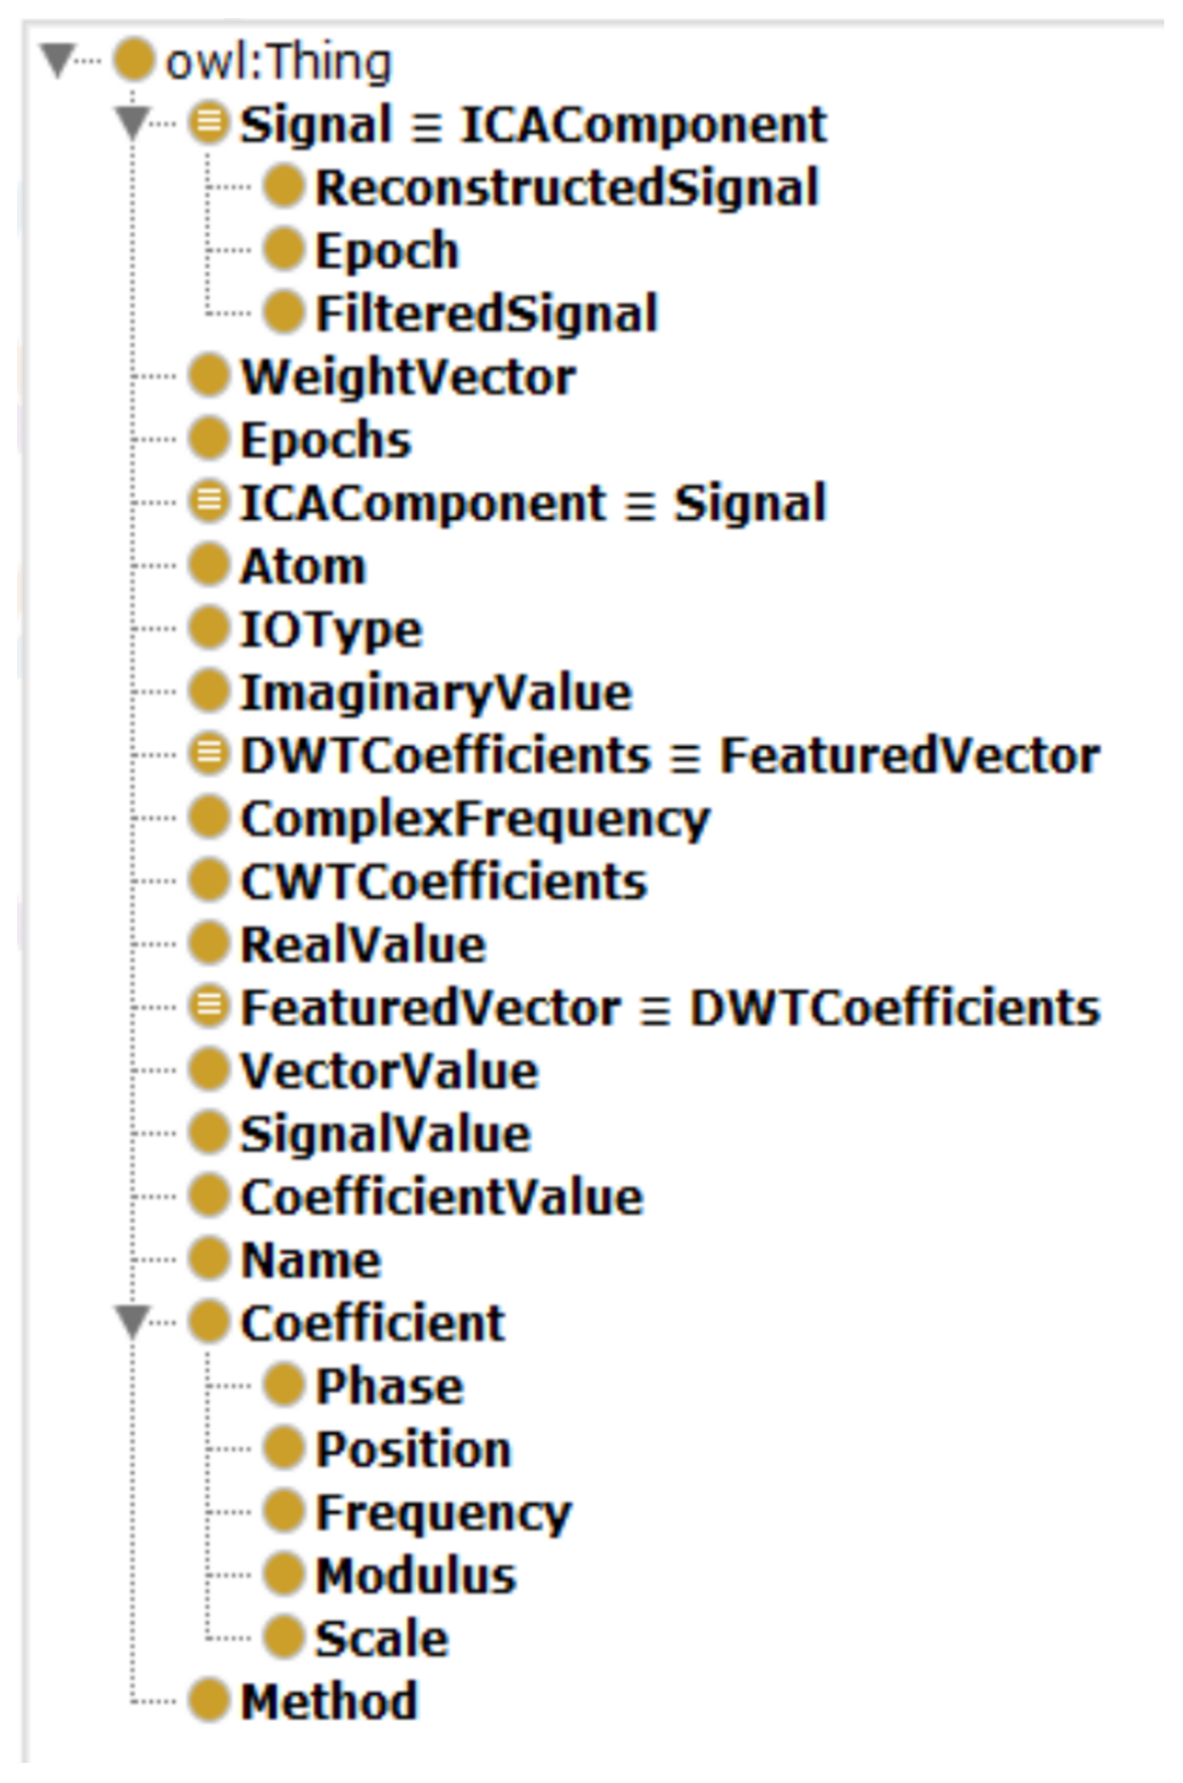
\epsfig{file = classTree.eps, width = 6 cm}}
  \caption{Tree of classes}
  \label{fig:classTree}
 \end{figure}

\section{\uppercase{Conclusions}}
\label{sec:conclusion}

\noindent This paper summarizes methods suitable for EEG/ERP signal
preprocessing and processing. It brings an introduction
to principles of these methods as well as their using
for ERP waveforms detection or artifacts removal.

Since complex data analyses often require using multiple methods sequentially, it is crucial to find suitable methods to achieve a goal. Therefore, we defined the set of metadata describing methods suitable for electrophysiology research.

Adding semantics to the methods in form of metadata allows checking both syntactic and semantic compatibility. Using the Semantic web technologies also enables processing metadata by machines. Therefore, we develop the ontology includes defined metadata. This brings an ability to develop automatic or semi-automatic workflow systems.

The presented ontology is also easily extendable. It allows reusing existing classes and properties, it also enables defining new classes and/or properties when necessary.

\subsection{Future Work}
\noindent We will annotate the input/output parameters of our methods with the terms defined in the ontology. It allows us to ensure the compatibility of methods while constructing workflows.

We also plan to develop a workflow suggestion system based on the presented ontology that will help users to find suitable methods while constructing workflows.


\section*{\uppercase{Acknowledgements}}

\noindent The work was supported by the UWB grant SGS-
2013-039 Methods and Applications of Bio- and
Medical Informatics.


\vfill
\bibliographystyle{apalike}
{\small
\bibliography{HEALTHINF2016}}



\vfill
\end{document}

